% ------------------------------------------------------------------------------
% Chapter 3 : Setup steps and Basic Usage Insight
% ------------------------------------------------------------------------------
\setlength{\parindent}{4em}
\setlength{\parskip}{1em}

In this section we will go through basics like performance measurement concept, tools to measure performance, LLVM, instruction set simulator(ISS) and basic learning techniques to understand the thesis. Performance of software on embedded hardware is essential in embedded product development. The measure question is how to measure performance of software on hardware. Here software maybe an application or operating system. Performance of application or operating system can be  analyzed and improved using performance monitoring features provided by embedded hardware. Now every modern hardware processor has Performance Monitoring Unit(PMU) on chip. PMU is on-chip hardware device that monitors the micro-architectural events. Events like cache hits, cache miss, cycles etc. Data collected from PMU can be use to observe the behavior of application or operating system on hardware processor. This collected data can be use to improve the performance. 

\par Performance monitoring events can be categorized in two types, one is hardware events and second is software events. Hardware events contain the events related to hardware like cycles, instructions, cache miss, cache hit etc. Where software events are related to software like page fault, segmentation fault, context switch etc. Performance monitoring hardware consists two components, performance event select registers and event counters. Performance event select registers are configuration registers to control what events to be monitored and how to monitor. Event counters registers, those count the number of events based on event select registers configuration. Also there are two approaches for performance monitoring, one is counting and other is event based sampling. Following figure \ref{fig:pmu} shows the block diagram of PMU in ARM Cortex A53 processor. 

\begin{figure}[h!]
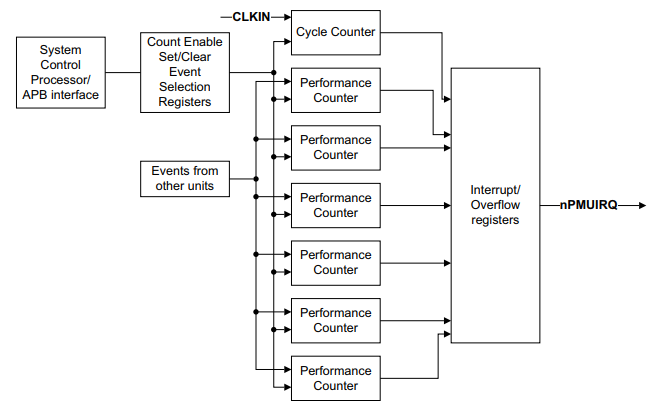
\includegraphics[width=14cm, height=10cm]{./images/pmu}
\centering
\caption{Block diagram of PMU in ARM Cortex A53 processor}
\label{fig:pmu}
\end{figure}

\section{Tools for Performance Measurement}
To evaluate the performance of software on hardware, variety of tools are available. These tools provide high level interface and analysis capabilities for performance monitoring hardware. The Performance Application Programming Interface (PAPI) tool suite [papi link] provides a common interface to performance monitoring hardware for many different processors like Alpha, ARM, MIPS, Pentium, PowerPC and etc. VTune Performance Analyzer [link for it] from Intel support performance monitoring on Intel's processor. PERF is performance analyzing tool in Linux, available from Linux kernel version 2.6.31 [link for perf]. OProfile[link for OProfile] is system-wide  statistical profiling tools for Linux to measure the performance of underlying hardware processor. ARM's Streamline Performance Analyzer provide in depth look of software performance on ARM processors. In this thesis, we are going to see tools like PAPI, PERF and Streamline Performance analyzer to evaluate the performance of software. In this thesis, we are focusing on hardware events and the performance data provided by these performance measurement tools measured on Raspberry Pi 3B board, which includes ARM Cortex A53 processor.

\subsection{PERF}
PERF is performance analyzing tool in Linux operating system and it is available from version 2.6+ of Linux kernel. PERF can accessed by userspace controlling utility, named 'perf'. PERF command line interface on Linux provides number of subcommands. PERF provides statictical data performance data of Linux kernel and user application. PERF supports hardware performance counters, software performance counters and tracepoints. PERF is based on 'perf\_events' interface. 

\par PERF Linux tool supports wide majority of events to provide the performance data. This tool can measure events from different sources using kernel interface. One source of events are kernel counters and these events are called software events like context switches, page-fault, alignment fault, emulation fault and etc. Another source of events is processor itself. PERF reads the events from hardware performance counter of PMU of processor. PERF provides the list micro-architectural events supported by it such as number of cycles, L1 cache miss, total instructions, branch mispredicted and many more.  Finally, the tracepoint events which are provided by kernel through 'ftrace' infrastructure.

\par One of the main feature of the PERF is that it allowed to select the specific core/s of processor using processor-wide mode. The performance data of specific core/s  can be collected for given application or operating system. Which had very significance in this thesis. It also creates the report of the collected sample data in file called 'perf.data'.It also possible with PERF to go more in granularity of instruction level with 'perf annotate'. 	PERF also provide the live analysis like Linux top command with processor wide feature. it is possible to measure the performance of application in userspace as well as kernel space. 

\par PERF provides subcommands on command line interface such as 'stat, record, report', etc. It is possible to get the list of software and hardware events supported by PERF using 'list' command for running embedded hardware processor. Following is the PERF usage on Raspberry Pi 3B board with Raspbian, Linux based operating system and we are measuring the performance of basicmath application from Mibench suite[] for single core i.e. second core of Cortex A53..


\begin{lstlisting}
$ sudo perf_3.16 state -e cycles,instructions,cache-misses,
 branches,branch-misses -C 2 ./runme_large.sh

# started on Wed Apr  4 14:02:59 2018 

Performance counter stats for 'CPU(s) 2':     
1,654,827,425      			cycles                        
1,397,787,969      			instructions              #    0.84  insns per cycle                    
3,528     	 				cache-misses                                                       
94,047,959     	 			branches                                                             
2,669,120    	 			branch-misses          #    2.84% of all branches              
2.445278109 seconds time elapsed
\end{lstlisting}

\subsection{PAPI}
PAPI is abbreviation for Performance Application Programming Interface. PAPI project is developed at University of Tennessee's Innnovative Computing Laboratory in Computer Science Department. This project was created to design, standardize, and implement a portable and efficient Application Programming Interface (API) to access the hardware performance counters found on most modern microprocessors[papi user guide]. PAPI provides an API to read hardware performance counter values for application running on processor. This data can be use to improve the performance of application or code. Similar kinds of APIs are available but PAPI provides stable API, documentation and upgrade it with features and different platforms. 

\par PAPI provides solid base for cross-platform tools. It provides standardize API. It is easy to use and freely available. It provides consistent interface and methodology to tool designers as well as application engineers to collect data from performance counters of PMU.  It provides near real time performance data between application and processor events. PAPI provides operating system independent access to hardware performance counters. 

\begin{figure}[h!]
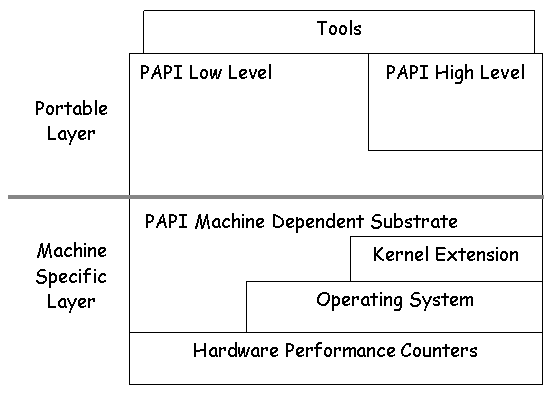
\includegraphics[width=12cm, height=8cm]{./images/papi}
\centering
\caption{Internal architecture of PAPI}
\label{fig:papi}
\end{figure}  

\par Above figure \ref{fig:papi} shows the internal architecture of PAPI. The architecture is divided into two parts, portable layer and machine specific layer. Portable layer has low level, high level and machine independent support functions. Whereas machine dependent layer consists of machine dependent functions and data structures. Layer also consists kernel extensions and operating system calls or assembly language to retrieve the data from counters of PMU. PAPI provides two interfaces, High level API and Low level API. High level API is easy to use and require less set-up but it has higher overhead and less flexibility. Considering that Low level API provides fine grained measurements, more control to interface and increase the functionality and efficiency. 

\par PAPI also provides command line interface event queries for existence of native or preset event to give more light about hardware supports specific events. Following code shows the PAPI API calls in code.  

\begin{lstlisting}
#include <papi.h>
#define NUM_EVENTS 2 

int main()
{
int Events[NUM_EVENTS] = {PAPI_TOT_INS, PAPI_TOT_CYC};
long_long values[NUM_EVENTS];
/* Start counting events */
if (PAPI_start_counters(Events, NUM_EVENTS) != PAPI_OK)
   handle_error(1); 
for (int i=0;i<1000:i++); 
if (PAPI_read_counters(values, NUM_EVENTS) != PAPI_OK)
   handle_error(1);
if (PAPI_stop_counters(values, NUM_EVENTS) != PAPI_OK)
   handle_error(1);
}
\end{lstlisting}

\par Following stats are showing the performance of Basicmath application from MiBench suite[]. Performance data is collected using PAPI API on Cortex A53 on single core that is core 2. 
\begin{lstlisting}
 $sudo ./runme_large.sh
 cycles:		1653593201,
 instructions:	1397640501,
 L2 cache miss:	2178,
 branches:	137950307,
 branch misses:	2668136
\end{lstlisting}

\subsection{Streamline Performance Analyzer}
Streamline Performance Analyzer is system-wide visualizer and profiler tool from ARM for ARMv7 and ARMv8 hardware targets. It generates the processor profile by reading the program counter at regular sample and collect the information about where processor spends its time. It collects the information of micro-architectural events from PMU of target hardware. Streamline gathers the performance data by communicating with software agent on target hardware. Streamline uses two communications agents, gator and barman. Gator is use for Linux targets whereas barman used for bare metal targets. 

\par In Streamline, best requisite set of hardware performance counters are used by default. But it is possible to change the configuration of hardware counters using Counter configurations dialog, which contains the list of available hardware performance counter for given specific target hardware. Streamline collects data in terms of samples and there are two modes of collecting samples in Streamline. One is fixed rate, where samples are collected in fixed intervals of time and this option is default in sampling method. Other method is Event-based sampling, where sampling is done on context switching or when an event occurs number of times.

\par Streamline provides Graphical User Interface (GUI). It shows captured data graphically. Streamline provides the functionality to capture data with counter configuration, start and stop of new captures of performance data. It provides live capture where in real time performance data is shown graphically in Streamline window for application being measured or profiled. It plots the counters in real time. After completion of the capture,capture information is shown in charts and details panel. Call paths in Streamline displays a hierarchy of functions, thread, processes. It also lists all functions in application called while capture. It also shows the core wise execution of thread and processes. Streamline also provide statistics line by line for source code. It also provides the string annotations and markers features which allows to add context to the information. Following image \ref{streamline} show the performance data collected for basicmath application from MiBench suite[] on Cortex A53 processor using Streamline performance analyzer. 

\begin{figure}[h!]
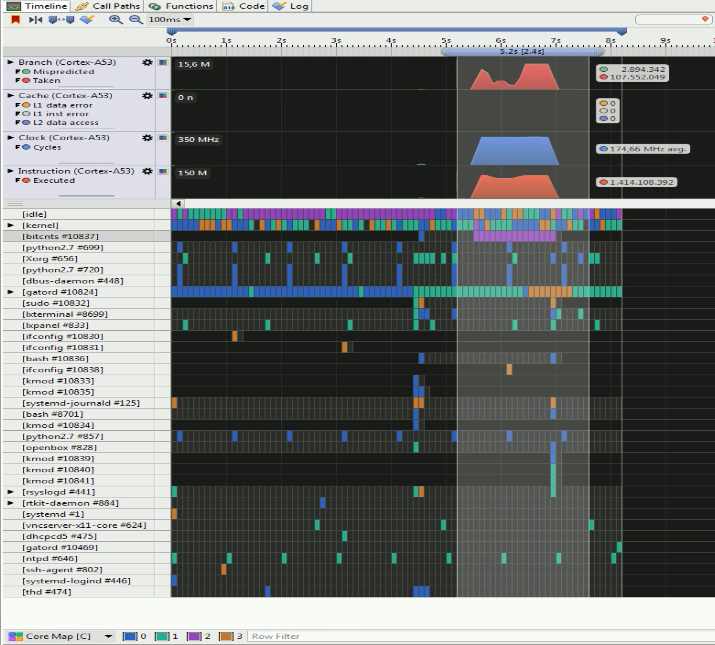
\includegraphics[width=16cm, height=12cm]{./images/streamline}
\centering
\caption{Timeline of basicmath application using Streamline Performance Analyzer}
\label{fig:streamline}
\end{figure} 

\section{Tools for Framework Development}
Apart from performance measurement tools, in this thesis we are also using tools which are freely available to use and create the framework for performance measurement. We are going to see LLVM compiler infrastructure project and Instruction Set Simulator(ISS) for create virtual simulation of hardware. 

\subsection{LLVM}
LLVM is collection of compiler and toolchain technologies used for development of front end and back end of compiler. Low level toolscahins like assemblers, debuggers, etc. LLVM started as a research project at University of Illinois. Initial motivation of LLVM was investigate dynamic compilation technique for static and dynamic programming languages[llvm.org]. LLVM is written in C++ language and it is designed for programs written in arbitrary programming language. Clang is LLVM native C/C++ compiler which provides more features than GCC and faster than GCC. Over last decade, LLVM is used as common infrastructure to implement runtime compiled languages, family of languages supported by GCC, Java, .NET, Python, Ruby, Scheme, etc. 

\par Traditional and popular design for compiler is divided into three major components, those components are the front end, the optimizer and the backend. The frontend component perform parsing of source code, checking the errors and represent the input code. The optimizer component try to improve the code by eliminating redundant computations and it is independent of language and target hardware architectures. The backend component converts the code into machine code compatible with target hardware architecture. One of the major implication of this design is that retargetability. If compiler uses common code representation for it's optimizer then backend can written for any target hardware architecture and frontend can be written for any source language. Which eliminate the wide number of compilers for each source language and for each hardware architecture. One of the successful implementation of this mode is GCC. It supports many frontends and backends and have wide community of contributors. 

\par  But there are limitations to this traditional approach. They are designed as monolithic applications for example GCC. Some pieces of libraries can not be reused. It has uncontrolling use of global variables, weakly enforced invariants, poorly-designed data structures, sprawling code base, and the use of macros that prevent the codebase from being compiled to support more than one front-end/target pair at a time. GCC suffers from layering problems and leaky abstractions: the back end walks front-end ASTs to generate debug info, the front ends generate back-end data structures, and the entire compiler depends on global data structures set up by the command line interface [chris lattner]. 

\par LLVM uses Intermediate Representation(IR) for code representation in compiler infrastructure. For any source code at frontend is converted into IR code and given to optimizer and output of the optimizer is also IR code which is faded to backend to create target machine code. You can see this behavior in following figure \ref{fig:llvm} of three phase structure of LLVM compiler. 

\begin{figure}[h!]
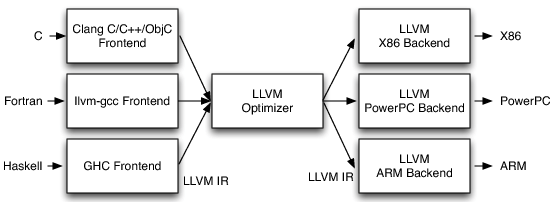
\includegraphics[width=12cm, height=6cm]{./images/llvm}
\centering
\caption{LLVM's three phase design}
\label{fig:llvm}
\end{figure}

LLVM IR is low-level Reduced Instruction Set Architecture(RISC) like virtual instruction set. We can see in this following example. 

\begin{lstlisting}
define i32 @add1(i32 %a, i32 %b) {
entry:
  %tmp1 = add i32 %a, %b
  ret i32 %tmp1
}

define i32 @add2(i32 %a, i32 %b) {
entry:
  %tmp1 = icmp eq i32 %a, 0
  br i1 %tmp1, label %done, label %recurse

recurse:
  %tmp2 = sub i32 %a, 1
  %tmp3 = add i32 %b, 1
  %tmp4 = call i32 @add2(i32 %tmp2, i32 %tmp3)
  ret i32 %tmp4

done:
  ret i32 %b
}
\end{lstlisting}

This is the LLVM IR for following C code. 

\begin{lstlisting}
unsigned add1(unsigned a, unsigned b) {
  return a+b;
}

unsigned add2(unsigned a, unsigned b) {
  if (a == 0) return b;
  return add2(a-1, b+1);
}
\end{lstlisting}

LLVM IR representation help to understand the code at machine level. LLVM also provide optimization at IR representation. LLVM is collection of libraries. LLVM also offers optimizations in terms of passes. LLVM passes is written in C++ class.  These passes traverse portion of program to either collect the information or transform the program. In this thesis we are going make use LLVM basic block pass to collect the performance data at basic block level. We will see it in detail in further chapters. LLVM also provide retargetablity for various source code languages and target architectures. It also provides capabiites by modular design such as when and where each phase of compiler runs, unit testing the optimizer and automatic test case reduction. 

\subsection{Instruction Set Simulator}
Instruction Ste Simulators(ISS) is simulation model and mostly coded into high level programming languages. This simulation models reflects the behavior of actual microprocessor/microcontroller. This simulation models can mimic various hardware architectures. ISS mimics the behavior by reading the assembly instructions and maintaining the processor registers. ISS are widely used for simulating the machine code of another hardware to check compatibility, monitoring and testing of machine code, testing and debugging of machine code, and to improve the performance. ISS are important in early embedded product release in market. It can help to simulate target hardware if it is not available in market or in prototype phase of development. Disadvantage of ISS is that they costly and oftenely they are slow. 

\section{Basic Learning Techniques}
It is possible to get mathematical relationship between input and respective output by observing the behavior. Mathematical statement or equation is formed using this one to one, one to many, many to one or many to many. Mathematical relationship can be formed by creating with support the dataset of this relationship. The dataset contains the history of wide range data of input and output. This analysis of of input output model helps to create statistical model that can be useful predict output for new every input using learned mathematical model and accurate dataset. 

\par This relationship between input and output is learned using Machine Learning. Machine learning techniques allows to form this relationship and create dataset to predict the result for every new input. This is done by without any explicit programming. Only important thing is create dataset of input and output that helps to understand the behavior of relationship between them. And mathematical model can be created to learned this relationship and used to predict the output. There basically three main machine learning techniques are available,they are, supervised learning, unsupervised learning and regression learning. Again in these three main learning techniques many sub-techniques are available. Obtained dataset in machine learning filed is called as training data. Which helps to understand the behavior. Machine learning technique is any application is depending upon relationship between input and output and use case. In some cases relationship is linear or in some cases data is in number of chunks.

\subsection{Regression}
Regression is most popular technique in the field of machine learning, in which linear regression and logistic regression are most widely used and known to data analytics.  There are also regression techniques are available. Regression is popular statistical techniques use for application of predictive modeling. In regression technique, relationship model is formed in between dependent variable and independent variable. These variable can be one or many. For example in annual sale prediction, sales is dependent variable whichis going to predicted whereas factors affecting the sales are independent variables, these can be one or many. 

\par In linear regression techniques, dependent variable is continuous in nature with respect to independent variable. And relationship between these variable is assumed to be linear in nature. Logistic regression method is used for classification. Classification can binary or multi-class classification. There are also different techniques such as lasso regression, ridge regression, 
and many more techniques are available. These techniques are depend upon application and analysis of the data. We will see in more detail in upcoming chapters.








